\documentclass[conference]{IEEEtran}

\usepackage[T1]{fontenc}
% STIX Two is a Times-compatible scientific serif with a matching math font, and
% it is the same family the figures are drawn in, so figure text and body text
% are one typeface. It is in TeX Live, so this builds anywhere.
\usepackage{stix2}
\usepackage{microtype}
\usepackage{graphicx}
\usepackage{booktabs}
\usepackage{float}
\usepackage{tabularx}
\usepackage{array}
\usepackage{amsmath}
\usepackage[numbers,sort&compress]{natbib}
\usepackage[dvipsnames]{xcolor}
\usepackage[hidelinks]{hyperref}
\usepackage{url}

\definecolor{linkblue}{HTML}{245A83}
\hypersetup{
  colorlinks=true,
  linkcolor=linkblue,
  citecolor=linkblue,
  urlcolor=linkblue,
  pdftitle={When Nominal False-Positive Rates Fail},
  pdfauthor={Nisaharan Genhatharan}
}

\newcommand{\kgw}{\textsc{KGW}}
\newcommand{\synthid}{\textsc{SynthID-Text}}
\newcommand{\fpr}{\mathrm{FPR}}
\newcommand{\variant}[1]{\texttt{#1}}
\renewcommand{\arraystretch}{1.15}
\setlength{\emergencystretch}{2em}
\newcolumntype{Y}{>{\raggedright\arraybackslash}X}

\title{When Nominal False-Positive Rates Fail:\\
Key- and Length-Dependent Null Behavior of\\
Canonical LLM Text Watermarks}

\author{\IEEEauthorblockN{Nisaharan Genhatharan}
\IEEEauthorblockA{\textit{UNSW Sydney}\\
Sydney, Australia}}

\begin{document}
\maketitle

\begin{abstract}
Keyed text-watermark detectors are usually described by a nominal false-positive
rate that follows from an idealized null: under the KGW green-list scheme, each
scored token is green with probability $\gamma$ independently of the others, so
the detector's $z$-statistic is standard normal and $z>2.326$ is a 1\% test. We
measure how far that null is from real text. Using exact reproductions of the
maintained KGW SelfHash and SynthID-Text references, ten frozen detector keys, and
10,000 unwatermarked SmolLM2-135M outputs scored at 128, 256, and 512 tokens, we
find that the nominal 1\% KGW threshold has an empirical false-positive rate that
depends on the key by two orders of magnitude: from 0.27\% to 48.4\% [47.4, 49.3]
at 512 tokens, growing with length for the inflated keys. The mechanism is simple.
Each key induces its own null green rate $p_k$ on real text (0.205 to 0.302 against
$\gamma=0.25$), the resulting shift in mean $z$ grows as $\sqrt{T}$ and predicts
the observed shift with $r=0.9999$, and over-dispersion adds the rest. The same
keys scored on 5,000 human-written passages reproduce the key ranking
(Spearman $\rho=+0.94$ [+0.76, +0.99]), so the bias is a property of the key
against ordinary token statistics, not of the generating model, which only
amplifies it. Rescoring those same passages under a second vocabulary, with the
keys, parameters and text held fixed, does not narrow the spread of
$p_k$, and over 128 keys the ranking does not survive the change
($\rho=+0.01$ [-0.16, +0.18]): the bias belongs to the pair of key and
vocabulary, and a rate measured for one tokenizer does not transfer to another. Per-key,
per-length empirical calibration on 5,000 outputs brings every held-out cell to
0.16\% to 0.96\%, at a cost in detection that a development-scale screen prices
at a few points. A prospective familywise acceptance rule fitted at its own
boundary nevertheless failed 18 of 60 cells, which we report as a design lesson on
validation margin. SynthID-Text's naive-independence reference stays near 1\%
throughout. All rates are reported with exact 95\% intervals.
\end{abstract}

\begin{IEEEkeywords}
language-model watermarking, false-positive control, empirical calibration,
KGW SelfHash, SynthID-Text, detector keys
\end{IEEEkeywords}

\section{Introduction}

A keyed text watermark lets a detector with the key test whether a text was
produced by a compatible generation process. In the green-list family introduced
by \citet{kirchenbauer2023watermark}, a secret key and the preceding context
partition the vocabulary at each step into a green list of fraction $\gamma$ and a
red list; generation favours green tokens, and the detector counts how many of the
$T$ scored tokens are green. The detector's operating point is stated through a
$z$-score whose null distribution is derived under one assumption: that in
unwatermarked text each scored token is green with probability exactly $\gamma$,
independently of every other. Under that assumption $z$ is standard normal and
$z>2.326$ is a one-sided 1\% test. Papers, toolkits, and deployment discussions
routinely quote this nominal rate as if it were a property of the scheme.

This paper measures how far that null is from the behaviour of a real detector on
real text, and explains the gap. We fix the implementation first: the canonical
KGW SelfHash and SynthID-Text adapters used here reproduce the maintained
reference implementations exactly, so nothing below can be attributed to a
mismatch. We then score 10,000 unwatermarked SmolLM2-135M-Instruct outputs at
three prefix lengths with ten frozen detector keys per scheme, report every rate
with an exact 95\% interval, and fit nothing.

That the i.i.d.\ assumption fails on real text is not new, and it is important to
be precise about what was already established. \citet{fernandez2023bricks}
demonstrated the failure at scale, over ten master keys and 100{,}000 Wikipedia
sequences of 256 tokens at the same $\gamma=0.25$, and attributed it to repeated
hashing contexts; their remedy is a non-asymptotic test together with a rectified
scoring rule that skips repeated contexts. \citet{cai2025collision} give the
general theory of that dependence. Both accounts locate the problem in dependence
between scored positions.

Two things follow that have not been shown. First, a second and separate effect
survives once dependence is handled: each key colours a different fraction of
ordinary text green, so the null mean is displaced rather than merely
over-dispersed. This is not a fine distinction. The canonical adapter measured
here already applies the rectified scoring of \citet{fernandez2023bricks},
skipping repeated contexts, and the nominal 1\% threshold still yields a 48.4\%
false-positive rate on the worst of ten keys. Second, the earlier measurements
pool their keys. A spread from 0.27\% to 48.4\% is invisible in an aggregate over
ten keys, and the aggregate is the one quantity a deployment cannot use, because a
deployment holds a single key. What is new here is that the failure is a mixture
over keys rather than a uniform bias, that its size and sign are fixed by the key
together with the tokenizer's vocabulary, that it grows with length instead of
averaging out, and what correcting it costs in detection. Those are this paper's
contributions, in order of evidential strength.
\begin{enumerate}
  \item \textbf{The nominal 1\% KGW threshold is key- and length-dependent.}
  Across ten keys at 512 tokens the empirical false-positive rate spans 0.27\% to
  48.4\% [47.4, 49.3], $n=10{,}000$ per cell; 20 of 30 key-by-length cells exceed
  1\% and the inflated keys get worse with length (Section~\ref{sec:c1}). Which
  key inflates is not portable: a Qwen2.5 replication fails different keys.
  \item \textbf{The mechanism is a key-specific null green rate.} Each key colours
  a different fraction $p_k$ of real text green, 0.205 to 0.302 against the assumed
  0.25. Substituting $p_k$ for $\gamma$ in the detector's own formula predicts the
  mean null $z$ of all 30 cells with $r=0.9999$, and the shift grows as $\sqrt{T}$.
  Over-dispersion adds a second, smaller effect. Repetition is not the driver
  (Section~\ref{sec:c2}).
  \item \textbf{The bias belongs to the key and the vocabulary, not the model.}
  The same keys on 5,000 human-written passages give the same ordering of $p_k$
  (Spearman $\rho=+0.94$) and the same worst key, with smaller inflation
  (Section~\ref{sec:c3}). Rescoring those same passages under a three-times-larger
  vocabulary does not narrow the spread of $p_k$, and over 128 keys the ranking
  does not survive ($\rho=+0.01$ [-0.16, +0.18], against
  $+0.94$ [+0.76, +0.99] within one vocabulary), with the model, keys, parameters
  and text all held fixed. The model amplifies the bias but does not choose which key carries it
  (Section~\ref{sec:c3b}).
  \item \textbf{Per-key, per-length empirical calibration works, and it is
  affordable.} Thresholds fitted once on 5,000 outputs and evaluated once on
  5,000 disjoint outputs give held-out rates of 0.16\% to 0.96\% in all 60
  scheme-by-key-by-length cells (Section~\ref{sec:c4}). A development-scale screen
  of 50 watermarked outputs per cell prices the cost at a median two points of
  detection at 512 tokens, gaining detection for the three keys whose threshold it
  lowers; that screen sizes the remedy and is not a detection claim
  (Section~\ref{sec:c4b}).
  \item \textbf{Fitting at an acceptance boundary leaves no familywise margin.} A
  prospective rule that required all 60 calibrated cells to pass an exact
  Bonferroni-controlled bound failed 18 cells, although no failed cell's point
  estimate exceeded 0.96\%. Twenty-eight of 30 KGW thresholds had been fitted at
  the maximum passing count, where a fresh cell passes with probability about
  55\% (Section~\ref{sec:c5}).
\end{enumerate}

The contribution is deliberately bounded. We do not claim that every
implementation called KGW or SynthID behaves alike, that the numbers transfer to
other models or languages, or anything about robustness to editing or
paraphrase. The detection rates we do report are development-scale and are there
to price the remedy, not to claim a detection result. What we claim is narrower and, we think, more
useful: for the named primitives, the nominal false-positive rate is not a
property of the scheme, and the evaluation that replaces it must be indexed by
key and by length.

\section{Related Work}

The area is surveyed by \citet{liu2025survey}; we situate this paper against the
strands it touches.

\paragraph{Keyed green-list watermarks.}
\citet{kirchenbauer2023watermark} introduced the green-list scheme and its
$z$-test detector. The follow-up reliability study formalized context-dependent
hashing, the SelfHash variant, repeated-context handling, and the dependence of
detection on observed length \citep{kirchenbauer2024reliability}. Both derive the
detector's null from the i.i.d.\ Bernoulli($\gamma$) assumption examined here.
\citet{zhao2023unigram} fix the green list independently of context (Unigram) and
prove robustness guarantees under the same style of null.
\citet{fernandez2023bricks} observed that the assumption fails on real text and
proposed corrected statistics. Their evidence is large and already human-written:
ten master keys against 100{,}000 Wikipedia sequences of 256 tokens at the same
$\gamma=0.25$, with the inflation attributed to repeated hashing contexts and
remedied by a non-asymptotic test together with a scoring rule that skips them.
\citet{cai2025collision} give the general theory of that collision-induced
dependence. Our measurements begin where those leave off, in three ways. We apply
their rectified scoring rather than comparing against its absence, and the
inflation persists. We decompose by key instead of pooling, which is what turns a
known aggregate failure into a spread of two orders of magnitude across the keys a
deployment might actually hold. And the human-text result here is not the first
null measured on human text, which theirs already was, but the first \emph{paired}
one: the same keys on human and model text, asking whether the ranking of $p_k$ is
preserved (Section~\ref{sec:c3}).

\paragraph{Distortion-free and cryptographic constructions.}
\citet{kuditipudi2023robust}, \citet{christ2023undetectable} and
\citet{hu2024unbiased} construct watermarks whose output distribution matches the
unwatermarked model and whose
detectors have exact or provable null behaviour by design. SynthID-Text
\citep{dathathri2024synthid} uses context-dependent seeding and tournament
sampling; its production evaluation covers quality, detection, edits, and
paraphrasing. These families do not share KGW's $z$-test null, which is why our
SynthID measurements are a reference rather than a failure and why the key effect
is a KGW-specific finding.

\paragraph{Benchmarks and toolkits.}
MarkMyWords \citep{piet2023markmywords}, WaterBench \citep{tu2024waterbench},
WaterPark \citep{liang2025waterpark}, and WaterJudge \citep{molenda2024waterjudge}
compare schemes on quality, detection, and tamper resistance; MarkLLM
\citep{pan2024markllm} packages many of them behind one interface. These
evaluations typically report detection at a scheme's nominal threshold with one
key. The present results show why that convention can misstate the operating
point by an order of magnitude and why the key schedule belongs in the reported
condition.

\paragraph{False-positive control.}
\citet{li2024statistical} develop pivotal statistics with explicit type-I error
control for watermark detection, and forensic-readiness work argues that error
rates must be established before watermark evidence is used in consequential
settings \citep{tamim2026forensic}. The operating points assumed elsewhere are
far stricter than the nominal 1\%: attack studies calibrate KGW detectors, the
SelfHash variant included, to false-positive rates of $10^{-3}$ and $10^{-6}$ on
the argument that a false accusation is expensive \citep{jovanovic2024stealing},
and evasion studies report detection at a fixed 1\% false-positive rate
\citep{krishna2023paraphrasing}. Both conventions presuppose that the nominal
rate is the delivered rate. \citet{fu2025multiuse} show a related but distinct
failure, in which the false-positive rate grows with the size of the key space
because many keys are tested at once; ours is present with a single key.
\citet{xie2025classroom} reach the same operational conclusion we do from a
different direction, replacing the nominal threshold with conformal calibration
for classroom AI-usage detection. On the negative side of the ledger,
\citet{sadasivan2025reliably} and \citet{pang2024nofreelunch} argue that detection
faces intrinsic limits under an adversary; our concern is the non-adversarial
case, where no attacker is present and the text is simply not watermarked. We supply the empirical side: how large the error is
for the most widely used detector, where it comes from, and what calibration
removes it.

\paragraph{Tokenization as a source of disparity.}
That a vocabulary partition can create systematic, unequal treatment is
established outside watermarking: tokenizers encode the same content at very
different lengths across languages, with consequences for cost and context budget
\citep{petrov2023tokenizers,ahia2023cost}, and tokenizer choice measurably changes
downstream model behaviour \citep{ali2024tokenizer}. Concurrent work audits watermarking across
languages and likewise concludes that detection thresholds must be calibrated per
deployment context rather than inherited \citep{nemecek2026crosslingual}. Neither
holds the key, the parameters and the text fixed while changing only the
tokenizer, which is what Section~\ref{sec:c3b} does to separate the vocabulary
from the model.

\section{Methods}

\subsection{Implementation Identity}

Before any null measurement, the validation suite pinned maintained reference
revisions for KGW and SynthID-Text, checked keyed token assignments, reproduced
aggregate detector scores from per-position traces, and compared generation step by
step. The canonical adapters used throughout this paper are
\path{kgw_author_selfhash_v1} (KGW SelfHash: $\gamma=0.25$, $\delta=2.0$, context
width 4, repeated contexts ignored) and \path{synthid_deepmind_hash_v1}. The stock
Transformers implementations were retained as separately named secondary variants
and are never pooled with canonical scores. The remaining SynthID top-$k$
boundary-tie difference was recorded as a decoder-policy difference.

\subsection{Null Corpus and Detector Statistics}

The primary null corpus is 10,000 unwatermarked continuations generated by the
pinned SmolLM2-135M-Instruct checkpoint (temperature 0.8, top-$k$ 40, 512 new
tokens) from 10,000 distinct Databricks Dolly prompts balanced by task category.
The corpus was produced as two disjoint 5,000-prompt splits for the calibration
study of Section~\ref{sec:calib}; because nothing in the nominal-threshold analysis
is fitted, both splits are pooled there. Every output was scored at its paired
128-, 256-, and 512-token prefixes by ten frozen detector keys per scheme. Keys
within a run therefore score the same texts and are paired, not independent.

For KGW, the detector statistic at a prefix is
\begin{equation}
  z = \frac{g - \gamma T}{\sqrt{T\gamma(1-\gamma)}},
  \label{eq:kgwz}
\end{equation}
where $g$ is the number of green tokens among the $T$ eligible scored positions
(SelfHash skips positions whose context has already been scored, so $T$ is below
the prefix length). The nominal one-sided 1\% threshold is $z>2.326$, which is
exact only if green membership is i.i.d.\ Bernoulli($\gamma$) under the null.
SynthID-Text's mean-$g$ detector has no nominal $z$; as a reference we report the
naive-independence normal approximation
$z=(\bar g-0.5)\sqrt{4\,d\,T}$ with $d$ watermarking depth, at the same 2.326
cutoff, labelled as such.

All rates are reported with exact two-sided 95\% Clopper--Pearson intervals
\citep{clopper1934confidence}. The exact interval is preferred to the Wald
interval throughout because the cells of interest are small-$p$ and, at the
smallest cells here, the Wald coverage is erratic in exactly the regime we report
\citep{brown2001interval}. No threshold in
Sections~\ref{sec:c1}--\ref{sec:c3} was chosen from the data.

\subsection{Secondary Null Runs}

Two earlier runs with the same ten keys are reported alongside the primary corpus:
a 500-output SmolLM2 development pilot, and an independent balanced 104-output run
with Qwen2.5-0.5B-Instruct in a clean environment. Both are development
diagnostics; their role here is to show that the primary result reproduces and
that which key inflates does not carry from one model and tokenizer to another.
That run varies the model and its vocabulary together; the fourth mechanism
analysis of Section~\ref{sec:mech-methods} separates them. A fifth detector-only
run widens the key sample rather than the corpus: 128 keys from the same
derivation, of which conditions 0--9 are the ten used throughout, scored on 1,500
of the human passages to give the marginal distribution of $p_k$
(Section~\ref{sec:c1b}).

\subsection{Mechanism Analyses}
\label{sec:mech-methods}

Four detector-only analyses of the stored token ids ask why the nominal
threshold fails. First, for each key $k$ and length we pool green counts over
eligible positions to estimate the null green rate $p_k$ and compare the observed
mean $z$ with the value Eq.~\eqref{eq:kgwz} implies when $\gamma$ is replaced by
$p_k$. Second, we relate each output's $z$ to its repeated-4-gram fraction to test
whether low-entropy repetition drives the inflation. Third, we score 5,000
de-duplicated human-written Dolly passages (\texttt{response} and \texttt{context}
fields, at least 128 tokens, selected by a hashed seed) with the same ten keys at
every prefix length each passage supports. Fourth, we rescore those same
passages under a second vocabulary, Qwen2.5-0.5B-Instruct at about 152k tokens
against SmolLM2-135M at about 49k, holding the ten hashing keys, the watermark
parameters and the text fixed, so that the tokenizer is the only thing that
varies. Eligibility at a given prefix length is itself tokenizer-dependent, so
each length is restricted to the passages both vocabularies support. No text is
generated and no model weights are loaded in any of these analyses.

\subsection{Empirical Calibration and One-Shot Confirmation}
\label{sec:calib}

The remedy we test is per-key, per-length empirical calibration. Thresholds were
fitted once on the 5,000-output calibration split for 60 cells (two schemes, ten
keys, three lengths) and then evaluated once on the disjoint 5,000-output
confirmation split. Comparisons were strictly $s>t$. KGW thresholds were indexed
by key and length; SynthID used one threshold per length equal to the maximum of
the ten key-specific calibration candidates, with every key still tested
separately at confirmation. The prospective acceptance rule was familywise: a cell
passed if its exact one-sided Clopper--Pearson upper bound at a Bonferroni-corrected
$\alpha=0.05/60$ \citep{dunn1961multiple} was at most 1\%, which allows at most 28 exceedances per cell, and the family passed
only if all 60 cells passed. Thresholds were frozen and hashed before the
confirmation split was generated, and no threshold was revised afterwards.

\section{Results}

\subsection{Canonical Parity Passed}

The canonical adapters reproduced both pinned maintained references exactly on the
tested detection fixtures and step-by-step generation checks, and aggregate scores
reconstructed exactly from exported per-position rows. Every result below is
therefore a property of the named primitives rather than of an implementation
mismatch.

\subsection{The Nominal 1\% KGW Threshold Is Key- and Length-Conditional}
\label{sec:c1}

Table~\ref{tab:nominal} and Figure~\ref{fig:nominal} give the empirical
false-positive rate of canonical KGW SelfHash at $z>2.326$ for all 30 key-by-length
cells, $n=10{,}000$ each. Point estimates exceed 1\% in 20 of 30 cells; the exact
95\% interval lies entirely above 1\% in 19 cells and entirely below 1\% in 8. The
spread across keys is two orders of magnitude at every length. Key 07 gives
19.1\%, 33.0\%, and 48.4\% [47.4, 49.3] at 128, 256, and 512 tokens; key 03 gives
0.32\%, 0.26\%, and 0.27\%. The median across keys rises from 3.5\% at 128 tokens
to 6.9\% at 512. Inflated keys therefore get worse with length while conservative
keys stay conservative, so no single length policy repairs the threshold. The
500-output pilot value of 47.0\% for key 07 at 512 tokens reproduces as 48.4\% at
$n=10{,}000$.

\begin{table*}[t]
  \centering
  \caption{Empirical false-positive rate (\%) of canonical KGW SelfHash at the
  nominal one-sided 1\% threshold ($z>2.326$) on 10,000 unwatermarked
  SmolLM2-135M-Instruct outputs per cell, with exact two-sided 95\%
  Clopper--Pearson intervals. Nothing is fitted.}
  \label{tab:nominal}
  \small
  \input{tables/table1-nominal-fpr}
\end{table*}

\begin{figure*}[t]
  \centering
  \includegraphics[width=\textwidth]{../figures/fig1-nominal-fpr-by-key.pdf}
  \caption{Canonical KGW SelfHash false-positive rate by frozen detector key and
  prefix length at the nominal $z>2.326$ threshold, $n=10{,}000$ unwatermarked
  SmolLM2 outputs per cell, exact 95\% intervals, log scale. Prefix length is
  shaded light to dark. Keys are categorical and are paired within texts, so the
  points are not independent across keys.}
  \label{fig:nominal}
\end{figure*}

Which key inflates does not carry across runs (Figure~\ref{fig:threeruns}). On
Qwen2.5-0.5B the worst keys are 04 and 05 at 41.3\% each, while key 07, the worst
key on SmolLM2, gives 5.8\%. The ten keys are the same bit strings in both runs.
That run changes the model and its tokenizer together and so cannot say which of
the two decides; Section~\ref{sec:c3b} separates them on identical text and finds
the vocabulary sufficient.

\begin{figure*}[t]
  \centering
  \includegraphics[width=\textwidth]{../figures/fig2-nominal-fpr-three-runs.pdf}
  \caption{The same ten keys at 512 tokens in three null runs: the primary
  SmolLM2 corpus ($n=10{,}000$), the SmolLM2 pilot ($n=500$), and the Qwen2.5-0.5B
  replication ($n=104$). The two SmolLM2 runs agree; the Qwen run inflates
  different keys.}
  \label{fig:threeruns}
\end{figure*}

SynthID-Text's naive-independence reference behaves differently: per-cell rates
range from 0.74\% to 1.58\%, 11 of 30 cells sit above 1\% by point estimate, and
seven have intervals entirely above 1\%. This is mild over-dispersion with no
key-specific bias, and we report it as a reference rather than as a SynthID
failure.

\subsection{Mechanism: Each Key Has Its Own Null Green Rate}
\label{sec:c2}

The per-key null $z$ distributions at 512 tokens (Figure~\ref{fig:zdist}) are
approximately normal but shifted and widened relative to the assumed $N(0,1)$:
mean $z$ runs from $-1.96$ (key 03) to $+2.24$ (key 07), and the standard
deviation from 1.26 to 1.58.

\begin{figure*}[t]
  \centering
  \includegraphics[width=\textwidth]{../figures/fig3-z-distributions.pdf}
  \caption{Null distribution of the KGW $z$ statistic at 512 tokens for each of the
  ten keys, $n=10{,}000$, against the assumed standard normal (solid) and the
  nominal cutoff (dashed). The shaded area past the cutoff is the mass this key
  puts beyond the nominal 1\% threshold; the percentage at each panel's top right
  is that cell's false-positive rate. Under the assumed null every panel would
  show the same 1\%.}
  \label{fig:zdist}
\end{figure*}

The shift has a simple source (Figure~\ref{fig:mechanism}). Each key induces its
own null green-token rate $p_k$ on this model's text, stable across lengths and
ranging from 0.205 to 0.302 at 512 tokens against the assumed $\gamma=0.25$.
Substituting $p_k$ for $\gamma$ in Eq.~\eqref{eq:kgwz} predicts a mean null $z$ of
$(p_k-\gamma)\sqrt{T}/\sqrt{\gamma(1-\gamma)}$, which grows as $\sqrt{T}$. The
observed mean $z$ across all 30 cells matches this prediction with $r=0.9999$. A
second, smaller effect is over-dispersion: the standard deviation of $z$ rises from
1.07--1.27 at 128 tokens to 1.26--1.58 at 512, which is why key 06
($p_k=0.249$) still shows 3.7\% at 512 tokens. A normal with each cell's observed
mean and standard deviation reproduces every cell's rate within 1.5 percentage
points.

\begin{figure*}[t]
  \centering
  \includegraphics[width=\textwidth]{../figures/fig4-key-green-rate-mechanism.pdf}
  \caption{(a) Null green-token rate $p_k$ for each key at 512 tokens, drawn from
  the assumed $\gamma=0.25$; colour marks which side of $\gamma$ the key falls on
  and the vertical bars are exact 95\% intervals. (b) Observed mean null $z$ for
  all 30 key-by-length cells against the value predicted from $p_k$ alone, with
  the identity line.}
  \label{fig:mechanism}
\end{figure*}

The failure is thus the standard $z$-test's i.i.d.\ Bernoulli($\gamma$) null being
wrong for real text, with the sign and size of the error set by which frequent
(context, token) pairs each key colours green. This is the phenomenon
\citet{fernandez2023bricks} documented for KGW-style detectors; here it is
quantified per key and per length on one pinned implementation.

Repetition is not the driver (Figure~\ref{fig:repetition}). The outputs are
repetitive (median repeated-4-gram fraction 0.23), but for the worst key the
correlation between $z$ and repetition is negative (Spearman $\rho=-0.29$): key 07
gives 63\% in the least repetitive quartile and 32\% in the most repetitive.
SelfHash already skips repeated contexts, which is why eligible positions average
363 of 512.

\begin{figure*}[t]
  \centering
  \includegraphics[width=\textwidth]{../figures/fig5-z-vs-repetition.pdf}
  \caption{(a) Mean null $z$ per key against prefix length on a log scale; the
  offsets grow as $\sqrt{T}$, away from zero in both directions, and only the
  keys ending beyond $|z|=1$ are coloured. (b) Density of per-output $z$ for key
  07 at 512 tokens against the output's repeated-4-gram fraction, $n=10{,}000$,
  with the median per decile; more repetition goes with lower $z$, not higher.}
  \label{fig:repetition}
\end{figure*}

\subsection{Human-Written Text Reproduces the Key Ranking}
\label{sec:c3}

If $p_k$ were a property of the generating model, human-written text under the
same keys would show a different ranking. It does not (Table~\ref{tab:human},
Figure~\ref{fig:human}). On 5,000 human-written Dolly passages, $p_k$ ranges from
0.216 to 0.280 at 512 tokens and tracks the model's $p_k$ key for key (Spearman
$\rho=+0.94$, $p=5\times10^{-5}$; Pearson $r=+0.96$ over ten keys). Key 07 is the
worst key in both populations and keys 03 and 04 the best in both. Human-text
rates at the nominal threshold are inflated in the same direction but by less:
key 07 gives 9.4\%, 16.4\%, and 25.5\% at 128, 256, and 512 tokens on human text
against 19.1\%, 33.0\%, and 48.4\% on model output, and 19 of 30 human cells lie
above 1\% by point estimate. Human text is also far less repetitive (median
repeated-4-gram fraction 0.016), and the inflation persists.

\begin{table*}[t]
  \centering
  \caption{Empirical false-positive rate (\%) at the nominal $z>2.326$ threshold
  on human-written Dolly passages (Human) and on unwatermarked SmolLM2 output
  (Model) for the same ten frozen KGW keys. Each human passage is scored at every
  prefix length it supports, so $n$ falls with length. The last rows give the
  range of the null green rate $p_k$ across keys and the cell sizes.}
  \label{tab:human}
  \small
  \input{tables/table2-human-null}
\end{table*}

\begin{figure*}[t]
  \centering
  \includegraphics[width=\textwidth]{../figures/fig6-human-vs-model-null.pdf}
  \caption{(a) False-positive rate at the nominal threshold and 512 tokens for the
  same ten keys on SmolLM2 output ($n=10{,}000$) and on human-written Dolly
  passages ($n=554$), exact 95\% intervals, log scale. The human intervals are
  wide because the 512-token human cell is small. (b) Per-key null green rate on
  human text against the same quantity on model output, with exact intervals on
  both axes; the diagonal is equality and the rules mark $\gamma=0.25$. Colour is
  the same side-of-$\gamma$ encoding as Figure~\ref{fig:mechanism}a.}
  \label{fig:human}
\end{figure*}

The key-specific bias is therefore a property of each key's green list against
ordinary English token statistics, not of SmolLM2's output distribution. The model
amplifies it, presumably because its low-entropy output concentrates mass on the
same frequent (context, token) pairs. A practical corollary is that a deployment
cannot repair the nominal threshold by calibrating on model text alone: human text
under the same key inflates too.

\subsection{The Ranking Is Specific to the Vocabulary}
\label{sec:c3b}

The Qwen2.5 replication of Section~\ref{sec:c1} changed the model and its
tokenizer together, so it cannot say which of the two decides that different keys
fail. A natural objection is also that a larger vocabulary should average the key
effect away. We separate the two by scoring the identical human passages of
Section~\ref{sec:c3} under a second vocabulary, Qwen2.5-0.5B-Instruct at about
152k tokens against SmolLM2-135M at about 49k, with the same ten keys, the same
watermark parameters and the same text. Only the tokenizer changes. Each length
is restricted to the passages both vocabularies support, giving $n=4{,}857$,
1{,}875 and 511 at 128, 256 and 512 tokens.

Neither the objection nor the model explanation survives
(Figure~\ref{fig:vocab}). The spread of $p_k$ across keys does not shrink under
the three-times-larger vocabulary; over these ten keys it is 0.065 under SmolLM2
against 0.077 to 0.082 under Qwen2.5, at every length. Nor is there evidence that the ranking survives: over ten keys at 512 tokens the
Spearman correlation of $p_k$ between the two vocabularies is $\rho=-0.15$
($p=0.68$), against $\rho=+0.94$ between human and model text under one
vocabulary. Ten keys is a small sample for a rank correlation, and we state the
limit rather than read a null out of a non-significant test: the 95\% interval on
$\rho$ here is $[-0.71, +0.53]$, against $[+0.76, +0.99]$ for the human-versus-model
comparison. What the data support is that the transfer is not of the strength seen
within one vocabulary, not that it is exactly zero. Key 07, the worst key in both populations of Section~\ref{sec:c3},
falls to sixth under the Qwen2.5 vocabulary and its rate at the nominal threshold
drops from 25.8\% to 3.5\%; key 05 rises from 6.5\% to 67.7\% and key 04 from
0.59\% to 31.3\%. Of 30 key-by-length cells, 19 exceed 1\% under the SmolLM2
vocabulary and 24 under the Qwen2.5 vocabulary, so the inflation itself is not
repaired by the larger vocabulary; it is only redistributed over different keys.

The key effect is therefore a property of the pair (key, vocabulary), not of the
key alone and not of the generating model. A green list is a partition of one
particular vocabulary, and the fraction of ordinary English it colours green
depends on both halves of that pair. This also sharpens the reading of the
Qwen2.5 replication: the different failing keys there need not indicate a
different frequent-pair distribution in a different model, because changing the
tokenizer alone is enough to reshuffle the ranking on text that does not change
at all.

\begin{figure*}[t]
  \centering
  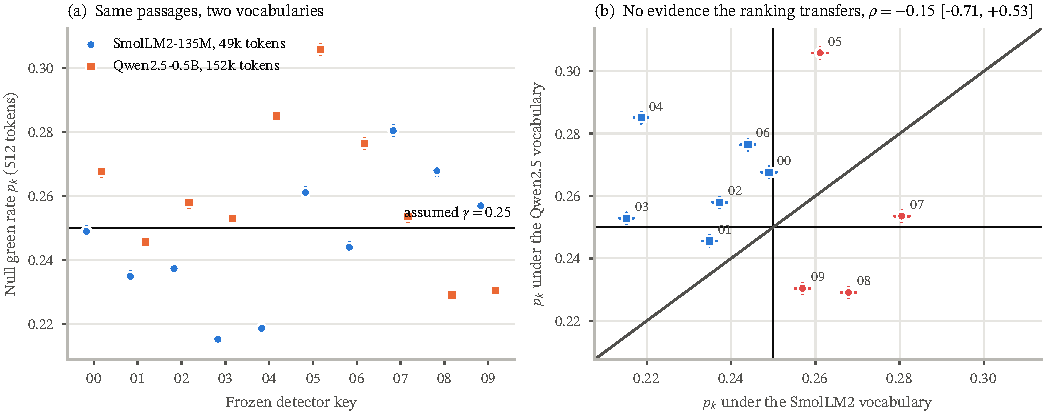
\includegraphics[width=\textwidth]{../figures/fig7-vocabulary.pdf}
  \caption{The same 511 human-written Dolly passages at 512 tokens, scored with
  the same ten frozen KGW keys and the same watermark parameters under two
  vocabularies. (a) Null green rate $p_k$ per key with exact 95\% intervals; the
  rule marks the assumed $\gamma=0.25$. The spread across keys does not narrow
  under the larger vocabulary. (b) $p_k$ under the Qwen2.5 vocabulary against
  $p_k$ under the SmolLM2 vocabulary, with exact intervals on both axes; the
  diagonal is equality and the rules mark $\gamma$. Colour is the same
  side-of-$\gamma$ encoding as Figure~\ref{fig:mechanism}a, taken from the
  SmolLM2 axis. Points fall off the diagonal in both directions; with ten keys the
  interval on $\rho$ is wide, so this shows the absence of strong transfer rather
  than an established zero.}
  \label{fig:vocab}
\end{figure*}

Ten keys cannot settle a rank correlation, so we repeated the comparison over the
128 keys of the sweep described below. Both vocabularies score an identical set of
passages at an identical set of prefix lengths: the run filters candidates on
joint eligibility under both tokenizers, without which the two legs select
different passages and the comparison is not paired. This widens the key sample
for the paired comparison itself, not only for the marginal distribution of $p_k$.

The wider sample narrows the interval enough to make the null informative
(Figure~\ref{fig:vocabsweep}). The correlation is indistinguishable from zero at
every length, and the interval is now narrow enough to exclude even a moderate
one: $\rho=+0.01$ $[-0.16, +0.18]$ at 128 tokens over 800 passages, $+0.01$
$[-0.16, +0.19]$ at 256 over 313, and $-0.02$ $[-0.19, +0.15]$ at 512 over 93.
The half-width of the interval falls from 0.63 at ten keys to 0.17 at 128, a
factor of 3.6. Ten keys admitted everything from a strong negative to a strong
positive correlation; 128 keys rule out any transfer stronger than weak. The
ranking of keys by $p_k$ does not carry across a change of vocabulary. The spread
itself is unchanged rather than widened: over 128 keys it is 0.098 under SmolLM2
against 0.100 under Qwen2.5 at 128 tokens, and the two are within 0.01 of each
other at all three lengths, so the ten-key impression that the larger vocabulary
widens the spread does not survive the larger sample. What survives is the claim
that matters for the objection: the larger vocabulary does not average the key
effect away.

\begin{figure*}[t]
  \centering
  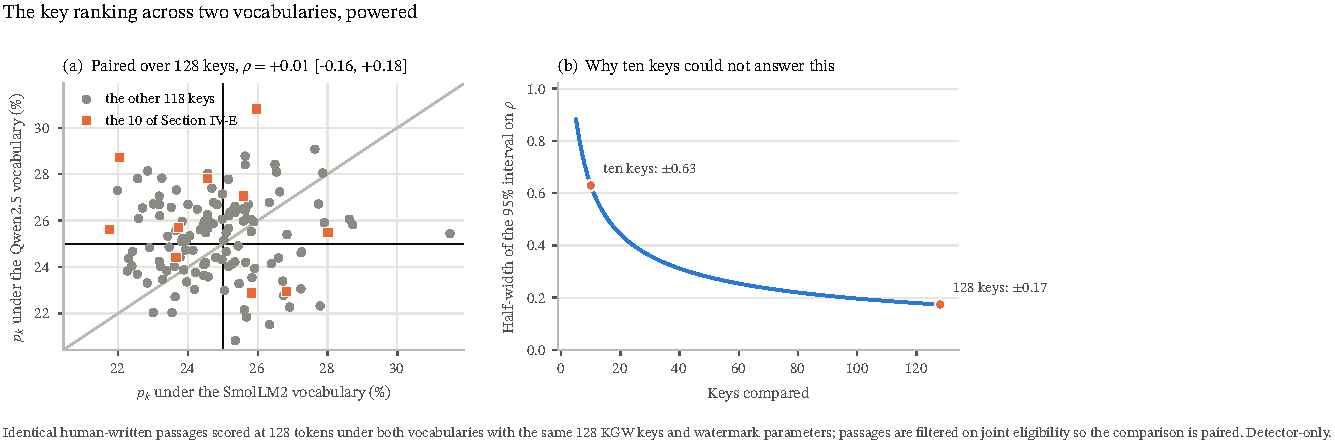
\includegraphics[width=\textwidth]{../figures/fig8-vocabulary-sweep.pdf}
  \caption{The paired cross-vocabulary comparison of Figure~\ref{fig:vocab},
  repeated over 128 keys at 128 tokens on the 800 passages both vocabularies
  support. (a) $p_k$ under the Qwen2.5 vocabulary against $p_k$ under the SmolLM2
  vocabulary; the ten keys used throughout the paper are marked, and fall inside
  the wider population rather than beside it. The diagonal is equality. The cloud
  is round: $\rho=+0.01$ $[-0.16, +0.18]$. (b) Half-width of the 95\% interval on
  a Spearman $\rho$ as a function of the number of keys compared, marking ten and
  128. At ten keys the interval spans $\pm0.63$ and can exclude almost nothing,
  which is why Figure~\ref{fig:vocab} supports only the absence of strong
  transfer; at 128 it spans $\pm0.17$.}
  \label{fig:vocabsweep}
\end{figure*}

\subsection{How Much of the Key Space Is Affected}
\label{sec:c1b}

Ten keys establish that the effect exists and that its ranking is stable, but not
how much of the key space carries it. We widened the sample with the same
derivation, so conditions 0--9 reproduce the ten used throughout the paper and
appear inside the distribution rather than beside it. The sweep scores 128 keys
against 1,500 human-written passages from the corpus of Section~\ref{sec:c3},
detector-only and KGW alone.

The spread is not a property of the ten (Figure~\ref{fig:sweep}). Across 128 keys
$p_k$ runs from 0.217 to 0.315 at 128 tokens and from 0.216 to 0.319 at 512,
against the assumed 0.25, with a median of 0.248 and 44.5\% of keys above
$\gamma$. The ten keys of Section~\ref{sec:c1} sit inside that distribution and,
if anything, slightly below its centre: their median $p_k$ at 128 tokens is 0.250
against 0.248 for all 128. Nothing about them was extreme.

At the nominal threshold the consequence is a majority effect rather than a tail
one. At 128 tokens, where every key is scored on all 1,500 passages, the
empirical false-positive rate runs from 0.13\% to 30.0\% with a median of 1.60\%;
88 of 128 keys (69\%) sit above the nominal 1\% by point estimate, and 68 (53\%)
have an exact 95\% lower bound that also clears it. At 512 tokens, where 179
passages per key reach that length, the range is 0\% to 82.1\% with a median of
2.23\%, 91 keys (71\%) above 1\% by point estimate and 57 (45\%) by lower bound.
The per-key intervals are wider at 512 because the cell is smaller, which is why
the conservative count falls while the point estimate rises. The worst key in the
sweep is worse than the worst of the original ten: 82.1\% against 48.4\%.

The practical reading is that a deployment drawing a key at random is more likely
than not to operate above the false-positive rate its detector advertises, and
that roughly half of all keys can be shown to do so from 1,500 passages alone.
This does not weaken the case for measuring $p_k$; it removes the possibility
that the ten keys of Section~\ref{sec:c1} were an unlucky draw.

\begin{figure*}[t]
  \centering
  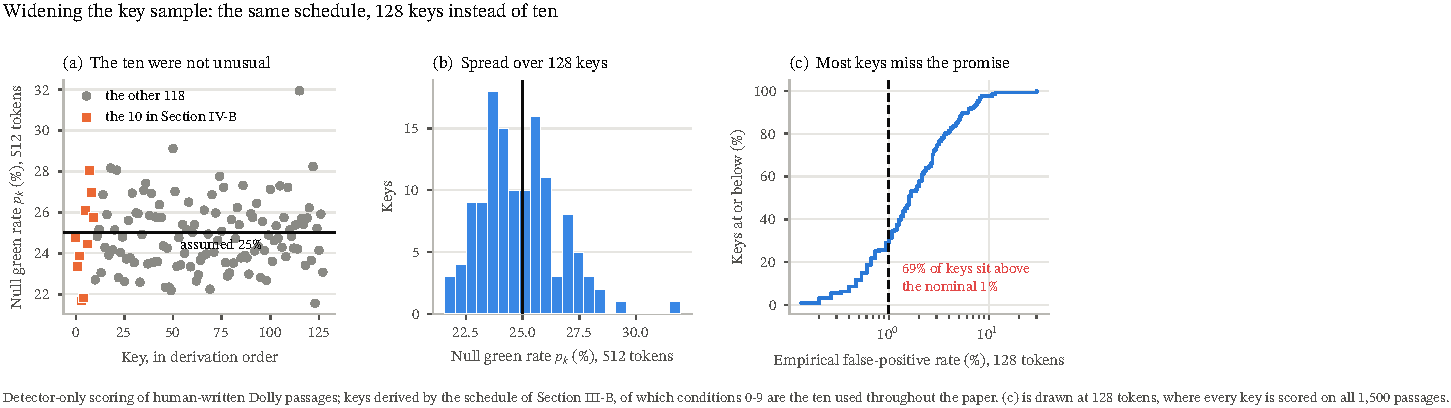
\includegraphics[width=\textwidth]{../figures/fig9-key-sweep.pdf}
  \caption{The same key schedule extended from ten conditions to 128, scored
  detector-only on 1,500 human-written Dolly passages. (a) Null green rate per
  key at 512 tokens, with the ten keys used elsewhere in the paper marked; they
  are not outliers. (b) The marginal distribution of $p_k$ that ten keys could not
  show. (c) Empirical cumulative distribution of the false-positive rate at the
  nominal threshold, drawn at 128 tokens where every key is scored on all 1,500
  passages; the dashed rule is the 1\% the detector promises.}
  \label{fig:sweep}
\end{figure*}

\subsection{Per-Key, Per-Length Calibration Brings Held-Out Rates Below 1\%}
\label{sec:c4}

Per-key empirical thresholds are not a new device: \citet{aremu2025forgery} fit
them from unwatermarked nulls, one per key, as a component of a defence against
watermark forgery. What has not been shown is that they are \emph{necessary} for a
single key at the nominal operating point, which is what the spread in
Section~\ref{sec:c1} implies and what the held-out rates below confirm. The
distinction matters for a second reason: that work assumes non-target keys give
approximately zero-mean scores under the null, an assumption about cross-key
scoring rather than about same-key scoring of unwatermarked text, and our
measurements bear only on the latter.

Appendix Table~\ref{tab:a1-kgw} and Table~\ref{tab:a1-synthid} list all 60
calibrated cells. Fitted KGW thresholds at 512 tokens range from $z=1.49$ (key 03)
to $z=6.40$ (key 07) against the nominal 2.326. On the disjoint confirmation split
the held-out false-positive rate of the once-fitted thresholds lies between 0.16\%
and 0.96\% in every cell, with no cell above 1\% by point estimate; the worst cell
is key 03 at 512 tokens, 0.96\% [0.71, 1.27]. KGW cells range 0.24\% to 0.96\% and
SynthID cells 0.16\% to 0.66\%. Empirical calibration at $n=5{,}000$ per cell thus
delivers the operating point the nominal threshold promised, provided the
threshold is indexed by key and length.

\subsection{What Calibration Costs in Detection}
\label{sec:c4b}

A per-key threshold that is far above the nominal one invites an obvious
objection: for key 07 at 512 tokens it sits at $z>6.40$ against a nominal
2.326, and a threshold that high might detect nothing. We can answer this from
stored scores. A 1{,}000-output development screen generated watermarked text
under the same model, the same watermark configuration and the same ten-key
schedule, so the thresholds frozen on the null's calibration split apply to it
unchanged. Those thresholds were fitted on unwatermarked text alone, so using
them on watermarked text is not circular. Detection rate here is the fraction of
watermarked outputs scoring above the threshold under their own key, on 50
outputs per cell.

Calibration does not disarm the detector (Figure~\ref{fig:detection}a). The
median detection rate across the ten keys falls from 99\% to 97\% at 512 tokens,
from 98\% to 95\% at 256, and from 96\% to 88\% at 128. For key 07 at 512 tokens
the false-positive rate falls from 48.4\% to 0.54\% while detection falls from
98\% to 96\%: an almost ninetyfold reduction in false positives for two points of
detection. The worst cell in the whole set is key 08 at 128 tokens, where
detection is 76\% [62, 87].

The correction also runs in both directions (Figure~\ref{fig:detection}b).
Calibration raised the threshold in 27 of 30 cells and lowered it in three, and
where it lowered the threshold, detection improved. Key 03 is the clearest case:
its null sits well below the assumed one, its calibrated threshold at 512 tokens
is $z>1.49$ rather than 2.326, and its detection rate rises from 96\% to 98\%; at
128 tokens it rises from 78\% to 86\%. Averaged over cells, calibration costs 4.2
points of detection where it raises the threshold and gains 5.3 points where it
lowers it. A conservative key is not harmless. It gives away detection power for
a false-positive rate below the one it was asked for, and only a key-conditional
threshold recovers that.

These are development-scale numbers on 50 outputs per cell, so the intervals are
wide, and they are not a confirmatory detection claim. They are sufficient to
answer the objection they were computed for: on this model and this watermark
configuration, the price of a correctly calibrated false-positive rate is a few
points of detection, not the loss of the watermark.

\begin{figure*}[t]
  \centering
  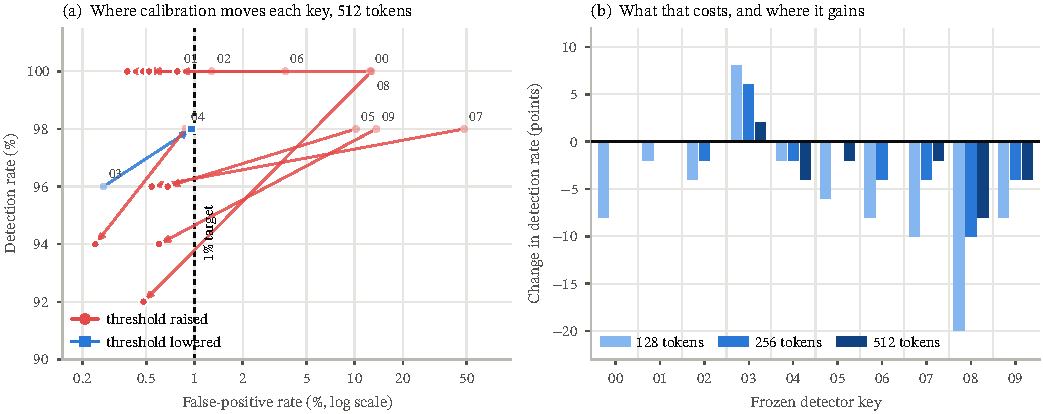
\includegraphics[width=\textwidth]{../figures/fig10-detection-tradeoff.pdf}
  \caption{(a) Operating point of each detector key at 512 tokens before and
  after per-key calibration, on a log false-positive axis. Arrows run from the
  nominal threshold to the calibrated one; labels sit at the nominal end. Colour
  marks whether calibration raised or lowered that key's threshold. (b) Change in
  detection rate from calibration, by key and prefix length. The three cells
  where the threshold fell are the three where detection improved. Detection
  rates are development-scale, 50 watermarked outputs per cell.}
  \label{fig:detection}
\end{figure*}

\subsection{Fitting at the Acceptance Boundary Leaves No Familywise Margin}
\label{sec:c5}

The same 60 cells were also subject to the prospective familywise rule of
Section~\ref{sec:calib}, and that rule failed: 42 cells passed and 18 did not
(14 KGW, 4 SynthID), even though every failed cell's point estimate lay between
0.58\% and 0.96\% and the largest Bonferroni-controlled upper bound was 1.48\%.
The reason is a design flaw rather than a held-out shift. Twenty-eight of 30 KGW
calibration cells were fitted at exactly the maximum passing count of 28
exceedances, and KGW averaged 27.9 exceedances in calibration against 27.7 in
confirmation (Figure~\ref{fig:margin}a). At a true rate equal to the boundary value
$28/5{,}000=0.56\%$, a fresh 5,000-output cell has only about a 55\% probability of
staying at or below the passing count, so a rule that requires all 60 cells to
pass was designed to fail. Prospective exact-binomial planning shows that more
observations narrow the penalty but do not remove the need for a true operating
rate below the target: under a conservative union bound, the largest true per-cell
rate compatible with 95\% whole-family pass probability rises from about 0.30\% at
5,000 observations to 0.74\% at 50,000 (Figure~\ref{fig:margin}b). These are
planning scenarios, not replacement thresholds. The failure is an instance of a
known hazard rather than a local accident: selecting a threshold on a calibration
sample and then asserting a risk guarantee requires the selection itself to be
treated as a multiple-testing problem, which is what the learn-then-test framework
formalizes \citep{angelopoulos2025learn}. Our rule performed the selection and the
guarantee at the same operating point, which is precisely the case that framework
is built to rule out.

\begin{figure*}[t]
  \centering
  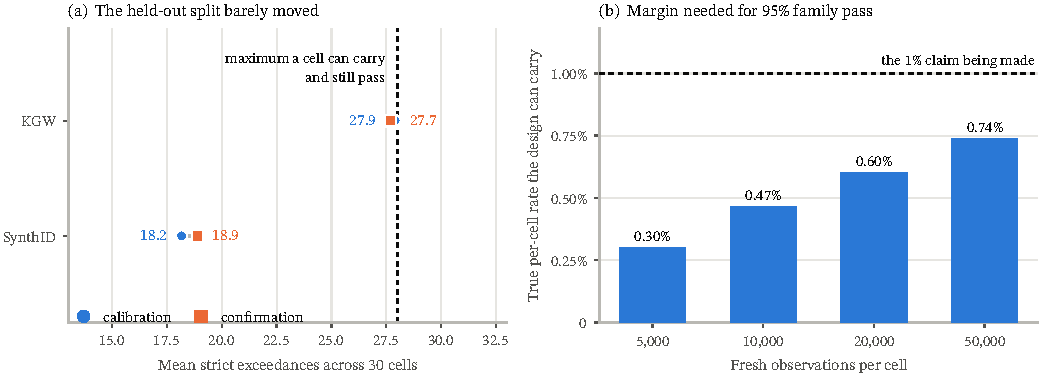
\includegraphics[width=\textwidth]{../figures/fig11-design-margin.pdf}
  \caption{(a) Mean strict exceedances across the 30 key-by-length cells of each
  scheme, on the calibration split and on the disjoint confirmation split, against
  the largest count a cell could carry and still pass. KGW's pair sits on the
  boundary and barely moves, so the gate failure is not a held-out shift.
  (b) Prospective union-bound planning: the largest true per-cell rate compatible
  with at least 95\% probability that all 60 cells pass, by fresh sample size.
  These are design scenarios, not replacement thresholds.}
  \label{fig:margin}
\end{figure*}

\section{Discussion}

\subsection{The Nominal Rate Is Not a Property of the Scheme}

The i.i.d.\ Bernoulli($\gamma$) null treats the green list as a random partition
of the vocabulary that ordinary text does not prefer. It is not. The partition is
uniform over vocabulary \emph{types}, while text is drawn over \emph{tokens}, and
token frequency is famously far from uniform \citep{piantadosi2014zipf}. A quarter
of the dictionary is therefore not a quarter of the words, and how far it departs
depends on which quarter the key selected. Each key's partition lands differently
on the frequent (context, token) pairs of English, so each key has its own $p_k$,
and the $z$-test amplifies the difference by $\sqrt{T}$. Two consequences
follow. A scheme-level false-positive rate is meaningless without
the key: for the same model and threshold, one key gives 0.27\% and another
48.4\%. And longer texts do not help: for an inflated key the nominal test gets
worse with length, because the bias grows with $T$ while the assumed standard
deviation does not.

That a population-level error rate can conceal large per-subject variation is not
a new phenomenon, only a new instance of one. Speaker recognition named it three
decades ago: aggregate error rates hid subjects whose individual rates were far
worse, the ``sheep, goats, lambs and wolves'' of the biometric menagerie
\citep{doddington1998zoo}, and face recognition later found error rates varying by
orders of magnitude across demographic groups under a single reported threshold
\citep{grother2019frvt}. The discipline's response in both cases was to stop
reporting one aggregate number and to report the conditioning variable instead.
For keyed watermark detection, the conditioning variable is the key.

\subsection{The Bias Belongs to the Key and the Vocabulary}

Human-written text under the same keys reproduces the ranking of $p_k$ and the
worst key, with smaller deviations from $\gamma$. This separates two explanations
that the model-only data could not: the key effect is not an artefact of a tiny,
repetitive model, and the model's contribution is to concentrate its output on
the pairs the key already favours. What the model does not decide is which key
fails. Scoring those same passages under a second vocabulary does not narrow the spread
of $p_k$, and over 128 keys the ranking does not survive it ($\rho=+0.01$
[-0.16, +0.18], Section~\ref{sec:c3b}), with the model,
the keys and the text held fixed. The
bias belongs to the key against the vocabulary it partitions; the model amplifies
it but does not choose it. The Qwen2.5 replication, which varies model and
vocabulary at once, is consistent with this and no longer needs a
frequent-pair explanation of its own. All of these facts argue for the same
practice. A deployment
should measure $p_k$, or equivalently the null rate, for its own key and its own
tokenizer on the text population it will score, including human text, rather than
inherit a rate from the scheme. A rate measured for a key is not portable to a
deployment that retokenizes, even when the key and the scheme are unchanged.

\subsection{Calibration Works; Familywise Guarantees Need Margin}

Per-key, per-length thresholds fitted once on 5,000 outputs delivered held-out
rates below 1\% in every cell. That is the practical remedy, and it needs nothing
beyond an unwatermarked corpus from the relevant population and a key schedule.
It is also cheap in the currency practitioners care about: a few points of
detection where the threshold rises, and more detection than the nominal
threshold gave where it falls.
The prospective familywise rule we also imposed failed, and the failure is
instructive. Selecting the least conservative threshold that satisfies a
calibration bound places every cell at the acceptance boundary, where a fresh
sample passes with probability near one half; requiring all 60 to pass then has
little chance of success however valid the multiplicity control. Protocols that
want a simultaneous guarantee should declare both the final error target and a
lower design rate that gives the family adequate pass probability, and should
size the calibration corpus to that design rate rather than to the target.

\subsection{What the Remedy Costs, and What a Cheaper One Would Need}
\label{sec:cheaper}

Per-key, per-length calibration invites the objection that it is expensive: a
fresh unwatermarked corpus for every key, length and tokenizer. The measurements
here make it cheaper than that. What the threshold needs is $p_k$, and $p_k$ is a
property of the key against a text population, not of any generation procedure.
Section~\ref{sec:c3} estimates it on human-written passages with nothing
generated and no model weights loaded, and Section~\ref{sec:c2} shows that
substituting the measured $p_k$ for $\gamma$ predicts the mean null $z$ of all 30
cells at $r=0.9999$. A deployment can therefore calibrate against any corpus that
resembles what it will score, including text it already holds, rather than
sampling thousands of generations per key.

A purely analytical correction would be cheaper still, and is the natural next
question: if the bias comes from the key's partition meeting the frequency
structure of ordinary text, predict $p_k$ from that structure and skip the corpus
pass. We do not offer one, and the variant measured here is the reason to be
careful. Under SelfHash the green list at each position depends on the candidate
token as well as the preceding context, so $p_k$ is not a marginal of the
unigram distribution over a fixed partition and cannot be recovered by reweighting
one. A context-only variant such as LeftHash is a more tractable starting point,
where the partition is fixed once the preceding token is known and $p_k$ becomes
an expectation over the bigram distribution. Whether that estimate is accurate
enough to replace a measured threshold is an open question this paper does not
settle; the released score files and the per-position trace exporter are the
material for testing it.

\subsection{Implications for Operational Use}

A keyed detector score is evidence of compatibility with a specified embedding
and detection process. It is not proof of authorship, misconduct, truth, or
intent. Operational claims should name the scheme variant, the key policy, the
length range, the null population on which the threshold was calibrated, the
uncertainty procedure, and the consequences of a false positive. On the evidence
here, a claim that rests on the nominal rate alone is unsupported for KGW-style
detectors.

\section{Limitations}

The primary experiments use small language models and pinned English prompt
sources; the size of the effect will differ for other models, languages, and
domains, although the mechanism does not depend on model size. Findings apply to
the explicitly named variants and parameter settings rather than to every
implementation called KGW or SynthID. The Qwen2.5 replication is small ($n=104$)
and establishes only that the failing keys differ. The vocabulary comparison of
Section~\ref{sec:c3b} uses two specific tokenizers, so it shows that the
vocabulary matters but cannot attribute that to vocabulary size as such rather
than to the particular merges each tokenizer learned; its ten-key cell at 512
tokens rests on the 511 passages both vocabularies support. The paired sweep that
widens that comparison to 128 keys scores 800 jointly eligible passages, so its
own 512-token cell rests on 93; the rank correlation there is the least
well-supported of the three lengths, and the 128-token cell, at 800 passages, is
the one to quote. The human-text null has 554
passages at 512 tokens, and its longer passages are largely reference text rather
than answers. SynthID-Text was evaluated against a naive-independence reference
because its mean-$g$ detector has no nominal $z$; its calibrated behaviour is in
Appendix~\ref{app:a1}. The detection rates in Section~\ref{sec:c4b} come from a
50-output-per-cell development screen, so they price the remedy at development
scale rather than confirming a detection claim. No robustness, attack or
paraphrase conclusion is available.

\section{Ethics and Responsible Use}

False accusations based on automated text detection can cause material harm, and
the harm is not distributed evenly: detectors built for this purpose have been
shown to misclassify non-native English writing at far higher rates than native
writing \citep{liang2023biased}. A keyed watermark detector is a different
mechanism, but the failure documented here has the same shape, an error rate that
is quoted as a single number and is in fact conditional on something the reader is
not told.
Accordingly, all claims in this paper remain conditional on named implementations,
keys, lengths, populations, and decision rules. We discourage use of watermark
detection as standalone evidence in disciplinary, employment, legal, or authorship
decisions. Raw generated continuations will be reviewed for memorized personal,
copyrighted, or unsafe content before any public release.

\section{Reproducibility and Artifact Availability}

The repository records frozen configurations, model and dataset revisions, prompt
selection manifests, key schedules, implementation fingerprints, per-position
audit formats, the frozen calibration thresholds, and the confirmation record.
Every table and figure in this paper is generated deterministically from stored
scores by a fixed script; no analysis required new generation. Model weights and
cached datasets are not redistributed; deterministic retrieval instructions and
immutable revisions are supplied instead.

The release is tag \texttt{v1} of
\url{https://github.com/nisaharan/when-nominal-false-positive-rates-fail}, and it
includes source code, tests, aggregate artifacts, prompt row identifiers and
hashes, tables, figures, and parity fixtures. It also carries the three compressed
score files the analyses read and the aggregated cells of both key sweeps, so a clone regenerates every table and figure in
this paper without generating any text; this was checked by cloning the release
and rebuilding the paper from it alone. The text-level tables carry token
statistics and a SHA-256 per text, never the text itself. Raw Dolly text requires
CC BY-SA 3.0 attribution and share-alike treatment. Raw generated continuations
and development runs that support no claim in this paper are retained privately
for audit and excluded from the reported package.

\section{Conclusion}

For canonical KGW SelfHash, the nominal 1\% false-positive threshold is neither
1\% nor a constant: it is a key- and length-dependent quantity that ranged from
0.27\% to 48.4\% on 10,000 unwatermarked outputs, because each key induces its
own null green rate on real text and the detector's $z$-test scales the resulting
bias by $\sqrt{T}$. Human-written text reproduces the key ranking, so the effect is
a property of the key rather than the model, and rescoring the same passages under
a second vocabulary leaves no evidence that the ranking survives the change, so
the quantity that matters is the pair of key and tokenizer. Widening the key
sample from ten to 128 shows this is not a property of an unlucky draw: 69\% of
keys sit above the nominal 1\% at 128 tokens and 53\% can be shown to from 1,500
passages alone, with the ten keys used here sitting unremarkably inside that
distribution. Empirical calibration indexed by key and length removes it, and it
needs a corpus rather than a generation campaign, because what the threshold
depends on is $p_k$. Evaluations and deployments of green-list watermarks should
therefore report the key schedule, the tokenizer and the calibration population as
part of the experimental condition, and should treat a nominal rate as a
hypothesis to be tested rather than a property to be quoted.

\section*{Acknowledgments}

The author acknowledges the maintainers of the KGW and SynthID-Text reference
implementations and the creators of the openly available model and dataset
artifacts used in this study.

\bibliographystyle{plainnat}
\bibliography{references}

\appendices
\section{Calibrated Per-Cell Held-Out False-Positive Rates}
\label{app:a1}

Table~\ref{tab:a1-kgw} lists the 30 canonical KGW cells and
Table~\ref{tab:a1-synthid} the 30 SynthID-Text cells. Each row gives the
threshold fitted on the calibration split, the strict exceedance count on both
splits, and the held-out rate on the confirmation split with its exact interval.
No cell's held-out point estimate exceeds 1\%.

\input{tables/tableA1-calibrated-cells}

\section{Data Sources and Evidential Role}

Table~\ref{tab:sources} lists every corpus the paper uses and what each one is
for. All scoring is detector-only on stored token ids.

\begin{table*}[t]
\centering
\small
\caption{Every corpus used in this paper and the role it plays. All scoring is
detector-only on stored token ids.}
\label{tab:sources}
\begin{tabularx}{\textwidth}{>{\raggedright\arraybackslash}p{0.26\textwidth}>{\raggedright\arraybackslash}p{0.16\textwidth}Y}
\toprule
Corpus & Size & Role \\
\midrule
SmolLM2-135M unwatermarked outputs & 10,000 & Primary null (Sections~\ref{sec:c1}--\ref{sec:c2}); also the calibration and confirmation splits of 5,000 each (Sections~\ref{sec:c4}--\ref{sec:c5}). \\
SmolLM2 development pilot & 500 & Secondary run; reproduces the primary key profile. \\
Qwen2.5-0.5B replication & 104 & Secondary run; shows that the failing keys differ once model and tokenizer both change. \\
Human-written Dolly passages & 5,000 & Human-text null (Section~\ref{sec:c3}) and the second-vocabulary comparison (Section~\ref{sec:c3b}); detector-only, no generation. \\
Human-written Dolly passages, key sweep & 1,500 & 128 keys from the same schedule (Section~\ref{sec:c1b}); detector-only, KGW only. \\
Human-written Dolly passages, paired vocabulary sweep & 800 & The same 128 keys under both tokenizers, on passages both vocabularies support (Section~\ref{sec:c3b}); detector-only, KGW only. \\
Watermarked positive screen & 1,000 & Detection rates at the calibrated thresholds (Section~\ref{sec:c4b}); development scale, 50 outputs per cell. \\
Development bias brackets & 1,400 & Out of scope; support no claim here. \\
\bottomrule
\end{tabularx}
\end{table*}

\section{Interpretation Checklist}

\begin{itemize}
  \item Every rate is conditional on the named variant, key, prefix length,
  threshold, and null population; none transfers to another key by default.
  \item A cell that failed the familywise rule in Section~\ref{sec:c5} is not
  evidence that its true rate exceeds 1\%; its point estimate is in
  Appendix~\ref{app:a1}.
  \item The SynthID-Text figures are a naive-independence reference, not a
  nominal claim by that scheme.
  \item Canonical and Transformers variant scores are never pooled.
  \item The detection rates are a development screen of 50 outputs per cell,
  reported to price calibration; they are not a confirmatory detection claim.
  \item Robustness to editing, paraphrase or attack was not evaluated.
\end{itemize}

\end{document}
